%-------------------------------------------------------------------------------
% midi_export
%-------------------------------------------------------------------------------
%
% \file        midi_export.tex
% \library     Documents
% \author      Chris Ahlstrom
% \date        2018-10-20
% \update      2021-04-14
% \version     $Revision$
% \license     $XPC_GPL_LICENSE$
%
%     This section discusses the details of the import/export functionality.
%
%-------------------------------------------------------------------------------

\section{Import/Export}
\label{sec:midi_export}

   This section explains the details of the MIDI import and export
   functionality, accessed by the main menu as noted in sections
   \ref{subsubsec:menu_file_import},
   \ref{subsubsec:menu_file_export}, and
   \ref{subsubsec:menu_file_export_midi_only}, on page
   \pageref{subsubsec:menu_file_import}.

\subsection{Import MIDI}
\label{subsec:midi_export_file_import}

   The \textbf{Import} menu entry imports an SMF 0
   or SMF 1 MIDI file as one or more patterns, one pattern per track, and
   imports them into the currently-active set.
   Even long tracks, that aren't short loops, are imported.
   The difference from \textbf{File / Open} is that the destination screen-set
   (bank) for the import can be specified, and the existing data in the
   already-loaded MIDI file is preserved.
   If the imported file is a
   \textsl{Seq66} MIDI file, it's proprietary sections will
   \textsl{not} be imported, in order to preserve the performance setup.
   The \textbf{Import} dialog is similar to the \textbf{Open} dialog.

   When imported, each track, whether music or information,
   is entered into its own loop/pattern box (slot).
   The import operation can handle reasonably complex files.
   When the file is imported, the sequence number for each track is
   adjusted to put the track into the desired screen-set.
   The import can place the imported data into any of the 32 available
   screen-sets.  Quite large songs can be built by importing patterns.

   Import also handles SMF 0 MIDI files.  It parcels out the SMF 0 data
   into sequences/patterns for each of the 16 MIDI channels.  It also puts
   all of the MIDI data into the 17th pattern (pattern 16), in case it is
   needed.  Note that this slot is used no matter which screen-set one imports
   the file into.  Bug, or feature?

\subsection{Export Song as MIDI}
\label{subsec:midi_export_file_export}

   Thanks to \textsl{Seq32}, exporting song performances (see the
   \textbf{Song Editor}) to standard MIDI format has been added.
   The \textbf{Export Song as MIDI} operation modifies the song in the
   following ways:

   \begin{itemize}
      \item Only tracks (sequences, loops, or patterns)
         \index{exportable}
         that are "exportable" are written.  To be exportable, a
         track must have triggers present
         in the \textbf{Song Editor}, and, \textsl{in the song editor}, it
         must not be muted.
      \item Each trigger generates the events, including repeats,
         offset-play of the events, and transposition.
         If there is a gap in the layout
         (e.g. due to an \textbf{Expand} operation in the
         \textbf{Song Editor}),
         then the corresponding gap in the events is exported.
         The result is a track that reconstructs the original
         playback/performance layout of that pattern.
         The events themselves are sufficient to play the performance exactly
         in any MIDI sequencer.
         The triggers are useful for further editing of the song/performance,
         so they are preserved in the triggers \textsl{SeqSpec} section, but
         they cover the whole song.
      \item Empty pattern slots between tracks are removed.
      \item No matter what set the original track was in, it ends up in the
         first set; sets are consolidated.
      \item Other additions, such as time signature and tempo meta events, are
         written in the same manner as for a normal \textbf{File / Save}
         operation.
   \end{itemize}

   The Export dialog is similar to the Open dialog; one will likely want to
   change the name of the file so as not to overwrite it.
   If there are no exportable tracks, the following message is shown:

\begin{figure}[H]
   \centering 
   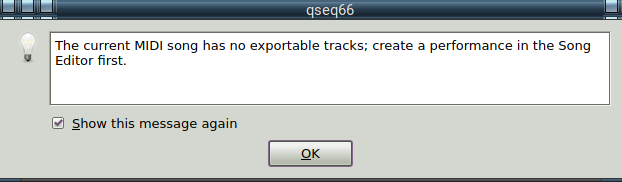
\includegraphics[scale=0.65]{main-menu/file/light-menu-file-song-unexportable.png}
   \caption{MIDI File Unexportable}
   \label{fig:midi_export_file_unexportable}
\end{figure}

   Once the file is exported, reopen it to see the results of the export.
   The following figure shows a before and after picture of the export, as
   seen in the song editor.

\begin{figure}[H]
   \centering 
   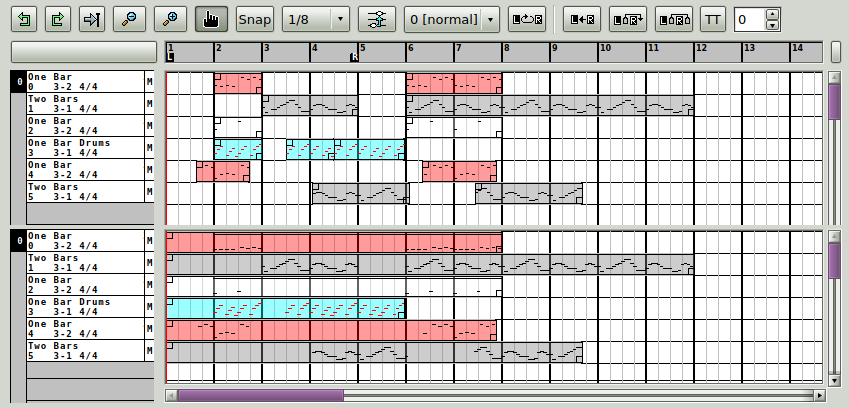
\includegraphics[scale=0.75]{song-editor/song-layout-sample-2.png}
   \caption{MIDI File Layout Before/After Export}
   \label{fig:midi_export_file_before_after}
\end{figure}
   
   The gaps in layouts in the song/performance data are reflected in the
   consolidated triggers.
   Here is the before/after triggers for pattern \#0, which was
   layed out with \textbf{Record Snap} \textsl{on}:

   \begin{verbatim}
       BEFORE                              AFTER
      Sequence #0 'One Bar'               Sequence #0 'One Bar'
      Length (ticks): 768                 Length (ticks): 5375
      trigger: 768 to 1535 at 768         trigger: 0 to 5375 at 5375
      trigger: 3840 to 5375 at 768        
   \end{verbatim}

   Note that 768, at PPQN = 192, is 4 beats (1 measure), while 5375 is 28
   beats (7 measures).
   For each of these triggers, the first number is the start of the trigger in
   PPQNs, the second is the end of the triger, and the third, called the
   "offset", is actually the length of the pattern.
   Note how the "AFTER"
   trigger consolidates the "BEFORE" triggers, starts at time 0, extends to
   the end of the last trigger, and has a length equal to the end of the
   trigger.

   Now here is the before/after triggers for pattern \#5, which was
   layed out with \textbf{Record Snap} \textsl{off}:

   \begin{verbatim}
       BEFORE                              AFTER
      Sequence #5 'Two Bars'              Sequence #5 'Two Bars'
      Length (ticks): 1536                Length (ticks): 6911
      trigger: 2344 to 3879 at 1536       trigger: 0 to 6655 at 6911
      trigger: 4944 to 6655 at 0
   \end{verbatim}

   6655 is a little over 34.5 beats, which is what the bottom grey trigger
   shows.
   6911 is almost 36 beats (9 measures).  Something to figure out.

\subsection{Export MIDI Only}
\label{subsec:midi_export_file_export_midi_only}

   Sometimes it might be useful to export only the non-sequencer-specific
   (non-SeqSpec) data from a \textsl{Seq66} song.
   For example, some buggy sequencers
   (hello \textsl{Windows Media Player})
   might balk at some SeqSpec item in the song, and refuse to load the MIDI
   file.
   For such cases,
   the \textbf{Export MIDI Only} menu item writes a file that does not contain
   the SeqSpec data for each track, and does not include all the SeqSpec data
   (such as mute groups) that is normally written to the end of the
   \textsl{Seq66} MIDI file.

%-------------------------------------------------------------------------------
% vim: ts=3 sw=3 et ft=tex
%-------------------------------------------------------------------------------
